\documentclass[12pt]{article}
\usepackage{amssymb,amsmath,amsthm}
\usepackage{tikz}
\usetikzlibrary{shapes,calc,arrows,positioning,backgrounds,patterns}
\usepackage{color}

\begin{document}

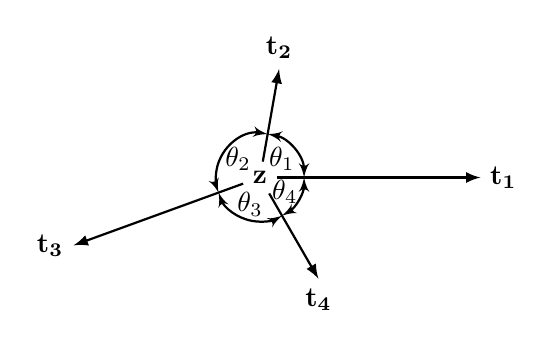
\begin{tikzpicture}[scale=0.7]
			\draw (0,0) node[] (z) {$\mathbf{z}$};
			\draw[-latex, thick] (z) -- (4,0) node (A) {};
			\node[right] at (A) {$\mathbf{t_1}$};
			\draw[-latex, thick] (z) -- ($(z)!0.5!80:(A)$) node[above] (B) {$\mathbf{t_2}$};
			\draw[-latex, thick] (z) -- ($(z)!0.9!200:(A)$) node[left] (C) {$\mathbf{t_3}$};
			\draw[-latex, thick] (z) -- ($(z)!0.53!300:(A)$) node[below] (D) {$\mathbf{t_4}$};
			\draw[latex'-latex', thick] ($(z.center)!.2!(A.center)$) arc (0:80:0.8);
			\draw[latex'-latex', thick] ($(z.center)!.2!80:(A.center)$) arc (80:200:0.8);
			\draw[latex'-latex', thick] ($(z.center)!.2!200:(A.center)$) arc (200:300:0.8);
			\draw[latex'-latex', thick] ($(z.center)!.2!300:(A.center)$) arc (300:360:0.8);
			\node at ($(40:0.8)!0.35!(z)$) {$\theta_1$};
			\node at ($(140:0.8)!0.35!(z)$) {$\theta_2$};
			\node at ($(250:0.8)!0.35!(z)$) {$\theta_3$};
			\node at ($(330:0.8)!0.35!(z)$) {$\theta_4$};
		\end{tikzpicture}

\end{document}